\documentclass[11pt]{article}
\usepackage{fontspec}
\usepackage{amsmath,amssymb,mathtools}
\usepackage[a4paper,margin=1in]{geometry}
\usepackage{enumitem}
\setlist[itemize]{noitemsep,topsep=2pt}
\setlist[enumerate]{noitemsep,topsep=2pt}
\usepackage{hyperref}
\usepackage{tikz}

\title{Lesson A1: Complex Numbers, Euler's Formula, and Rotations}
\author{Expanded, Step-by-Step Version for a Gifted Young Learner}
\date{}

\begin{document}
\maketitle

\section*{What we will build}
We link Euler's formula
\[
e^{i\theta}=\cos\theta+i\sin\theta
\]
to \emph{rotating points in the plane}. By the end you can:
\begin{itemize}
  \item move between rectangular form \(x+iy\) and polar form \(re^{i\theta}\),
  \item rotate about the origin by multiplying by \(e^{i\theta}\),
  \item rotate about \emph{any} center \(a\) using \(a+e^{i\theta}(z-a)\),
  \item do the same rotation using the \emph{rotation matrix} \(R_\theta\),
  \item run quick \emph{checks} (distances preserved, special angles).
\end{itemize}

\paragraph{Audience note.} We keep proofs tiny and hands-on. You will draw, compute, and check. (Parents/mentors: light calculator use is fine; exact values preferred at special angles.)

\bigskip
\hrule
\bigskip

\section*{Vocabulary, Symbols, and the “sent to” notation}
\begin{itemize}
  \item \(i\): the imaginary unit with \(i^2=-1\).
  \item \(z=x+iy\): a complex number; \(\Re z=x\), \(\Im z=y\). The point \((x,y)\) and the complex number \(x+iy\) are two names for the same thing.
  \item \(|z|=\sqrt{x^2+y^2}\): \emph{modulus} (distance from the origin).
  \item \(\arg z\): \emph{argument} (angle from the positive \(x\)-axis to \(z\); measured in radians).
  \item \(\overline{z}=x-iy\): \emph{conjugate}; \(z\overline{z}=|z|^2\).
  \item \textbf{“Sent to” notation.} When we write
  \[
     (x,y)\ \mapsto\ (x',y'),
  \]
  we mean: “our rule \emph{sends} the point \((x,y)\) to the new point \((x',y')\).” Read \(\mapsto\) as “goes to.”
\end{itemize}

\paragraph{Units tip (radians vs degrees).} We work in \emph{radians}. To convert: \(90^\circ=\pi/2\), \(60^\circ=\pi/3\), \(45^\circ=\pi/4\), \(30^\circ=\pi/6\). In general, \(\text{radians}=(\pi/180^\circ)\times\text{degrees}\).

\bigskip
\hrule
\bigskip

\section*{Core idea: Multiplying by \(e^{i\theta}\) rotates by \(\theta\)}
Let \(z=x+iy\). Using Euler’s formula,
\[
e^{i\theta}z=(\cos\theta+i\sin\theta)(x+iy)
=(x\cos\theta - y\sin\theta) + i\, (x\sin\theta + y\cos\theta).
\]
So the rule is
\[
(x,y)\ \mapsto\ \bigl(x\cos\theta - y\sin\theta,\ \ x\sin\theta + y\cos\theta\bigr).
\]
\textbf{Rotation matrix form.} Writing points as column vectors,
\[
\begin{pmatrix}x'\\y'\end{pmatrix}
=
\underbrace{\begin{pmatrix}
\cos\theta & -\sin\theta\\
\sin\theta & \ \cos\theta
\end{pmatrix}}_{\displaystyle R_\theta}
\begin{pmatrix}x\\y\end{pmatrix}.
\]

\paragraph{Two quick checks (distance is preserved).}
\begin{itemize}
  \item \emph{Complex check:} \(|e^{i\theta}|=1\Rightarrow |e^{i\theta}z|=|z|\).
  \item \emph{Coordinate check:}
  \(\ {x'}^2+{y'}^2=(x\cos\theta-y\sin\theta)^2+(x\sin\theta+y\cos\theta)^2=x^2+y^2\).
\end{itemize}
Rotations are \emph{rigid motions}: lengths and angles stay the same.

\bigskip
\hrule
\bigskip

\section*{Algorithm 1: Rectangular \(\leftrightarrow\) Polar (with quadrant adjustment)}
\textbf{Goal:} Write \(z=x+iy\) as \(z=re^{i\theta}\) with \(r\ge0\), \(\theta\in(-\pi,\pi]\).

\subsection*{Algorithm 1A: Rectangular \(\to\) Polar}
\begin{enumerate}[label=\textbf{Step \arabic*.}]
  \item Compute the modulus: \(r=\sqrt{x^2+y^2}\).
  \item Compute a \emph{base angle}: \(\theta_0=\arctan\!\bigl(\tfrac{|y|}{|x|}\bigr)\) (in \((0,\pi/2]\) if both nonzero).
  \item \textbf{Adjust to the correct quadrant} using the signs of \((x,y)\):
  \begin{itemize}
     \item Quadrant I (\(x>0,y>0\)): \(\theta=\ \ \ \theta_0\).
     \item Quadrant II (\(x<0,y>0\)): \(\theta=\pi-\theta_0\).
     \item Quadrant III (\(x<0,y<0\)): \(\theta=-(\pi-\theta_0)=\theta_0-\pi\).
     \item Quadrant IV (\(x>0,y<0\)): \(\theta=-\theta_0\).
     \item On axes: use \(\theta=0,\ \pm \tfrac{\pi}{2},\ \pi\) appropriately.
  \end{itemize}
  (On a calculator, \texttt{atan2(y,x)} does this automatically.)
  \item Report \(z=re^{i\theta}=r(\cos\theta+i\sin\theta)\). Sanity check: \(r\cos\theta\stackrel{?}{=}x,\ r\sin\theta\stackrel{?}{=}y\).
\end{enumerate}

\paragraph{Worked example (with quadrant adjust).}
Convert \(z=-\sqrt{2}+i\sqrt{2}\).
\[
r=\sqrt{(\sqrt{2})^2+(\sqrt{2})^2}=\sqrt{4}=2,\quad
\theta_0=\arctan\!\Big(\frac{\sqrt{2}}{\sqrt{2}}\Big)=\frac{\pi}{4}.
\]
Since \(x<0,y>0\) (Quadrant II), \(\theta=\pi-\frac{\pi}{4}=\frac{3\pi}{4}\).
Thus \(z=2e^{i3\pi/4}\).
\emph{Check:} \(2(\cos\frac{3\pi}{4}+i\sin\frac{3\pi}{4})=2(-\frac{\sqrt2}{2}+i\frac{\sqrt2}{2})=-\sqrt2+i\sqrt2\).

\subsection*{Algorithm 1B: Polar \(\to\) Rectangular}
Given \(z=re^{i\theta}\), compute
\[
x=r\cos\theta,\qquad y=r\sin\theta.
\]
\paragraph{Worked example.} \(z=3e^{i\pi/6}\Rightarrow x=3\cdot \tfrac{\sqrt3}{2}=\tfrac{3\sqrt3}{2},\ \ y=3\cdot \tfrac12=\tfrac{3}{2}\).

\medskip
\noindent\textbf{Practice A1 (do, then check):}
\begin{itemize}
  \item \(z=1+i\sqrt{3}\) \(\to\) \(re^{i\theta}\).
  \item \(z=5e^{-i\pi/3}\) \(\to\) \(x+iy\).
  \item \(z=-3i\) \(\to\) \(re^{i\theta}\) \emph{and} \(x+iy\) (tiny!).
\end{itemize}

\bigskip
\hrule
\bigskip

\section*{Algorithm 2: Rotate about the origin by \(\theta\) (complex multiplication)}
\textbf{Input:} \(z=x+iy\), angle \(\theta\). \quad
\textbf{Output:} \(z'=e^{i\theta}z\).

\begin{enumerate}[label=\textbf{Step \arabic*.}]
  \item (Rectangular method) Compute
  \[
  x'=x\cos\theta - y\sin\theta,\qquad
  y'=x\sin\theta + y\cos\theta.
  \]
  \item (Optional polar method) If \(z=re^{i\phi}\), then \(z'=re^{i(\phi+\theta)}\).
  \item \textbf{Checks:} \(|z'|=|z|\) and special-angle sanity (e.g.\ \(\theta=\pi\) flips signs).
\end{enumerate}

\paragraph{Worked example (rectangular).}
Rotate \(z=2-i\) by \(\theta=\pi/2\).
\[
x'=2\cdot 0 - (-1)\cdot 1=1,\qquad
y'=2\cdot 1 + (-1)\cdot 0=2.
\]
So \(z'=1+2i\). \(|z|=|z'|=\sqrt{5}\).

\paragraph{Workable example (you try).}
Rotate \(z=-2+2i\) by \(\theta=\pi/4\).
\emph{Hint:} \(\cos\frac{\pi}{4}=\sin\frac{\pi}{4}=\frac{\sqrt{2}}{2}\).
\emph{Answer (see Selected Answers):} page~\pageref{answersA1}.

\medskip
\noindent\textbf{Draw (graph paper).} Plot \(z\) and \(z'\). Use a right angle or rotate the paper to eyeball the turn. Distances to the origin should match.

\bigskip
\hrule
\bigskip

\section*{Algorithm 2M: Rotate using the rotation matrix \(R_\theta\)}
Same rotation, but do it by a clear matrix-times-vector computation.

\[
R_\theta=
\begin{pmatrix}
\cos\theta & -\sin\theta\\
\sin\theta & \ \cos\theta
\end{pmatrix},\qquad
\begin{pmatrix}x'\\y'\end{pmatrix}
=R_\theta\begin{pmatrix}x\\y\end{pmatrix}.
\]

\paragraph{Step-by-step dot products.}
\begin{enumerate}[label=\textbf{Step \arabic*.}]
  \item \textbf{Row 1 \(\cdot\) column:}
  \(\ x'=(\cos\theta)\cdot x + (-\sin\theta)\cdot y = x\cos\theta - y\sin\theta\).
  \item \textbf{Row 2 \(\cdot\) column:}
  \(\ y'=(\sin\theta)\cdot x + (\cos\theta)\cdot y = x\sin\theta + y\cos\theta\).
  \item \textbf{Check orthogonality:} \(R_\theta^\top R_\theta=I\) (explains length preservation).
\end{enumerate}

\paragraph{Worked example (matrix).}
Rotate \(z=(x,y)=(2,-1)\) by \(\theta=\pi/3\).
\[
R_{\pi/3}=\begin{pmatrix}\tfrac12 & -\tfrac{\sqrt3}{2}\\[2pt] \tfrac{\sqrt3}{2} & \tfrac12\end{pmatrix}.
\]
\[
x'=\tfrac12\cdot 2 + \Big(-\tfrac{\sqrt3}{2}\Big)\cdot(-1)=1+\tfrac{\sqrt3}{2},\quad
y'=\tfrac{\sqrt3}{2}\cdot 2 + \tfrac12\cdot(-1)=\sqrt3-\tfrac12.
\]
So \(z'=\bigl(1+\tfrac{\sqrt3}{2}\bigr)+i\bigl(\sqrt3-\tfrac12\bigr)\).
\emph{Distance check:} \({x'}^2+{y'}^2=2^2+(-1)^2=5\).

\medskip
\noindent\textbf{Practice A2M.}
\begin{itemize}
  \item Use \(R_{\pi/6}\) to rotate \((3,0)\). Compare with complex multiplication.
  \item Use \(R_{\pi}\) to rotate \((a,b)\). What do you notice?
\end{itemize}

\bigskip
\hrule
\bigskip

\section*{Algorithm 3: Rotate about a point \(a\) (not the origin)}
\textbf{Formula:}\ \ \(\displaystyle z_{\text{new}}=a+e^{i\theta}(z-a)\).

\begin{enumerate}[label=\textbf{Step \arabic*.}]
  \item Translate to the origin: \(w=z-a\).
  \item Rotate about the origin: \(w'=e^{i\theta}w\) (or \(w'=R_\theta w\)).
  \item Translate back: \(z_{\text{new}}=a+w'\).
  \item \textbf{Check:} \(|z_{\text{new}}-a|=|w'|=|w|=|z-a|\) (distance to center preserved).
\end{enumerate}

\paragraph{Worked example (complex and compass).}
Rotate \(z=3+i\) by \(\theta=\pi/3\) about \(a=1+i\).
\[
w=z-a=(3+i)-(1+i)=2,\quad
w'=2e^{i\pi/3}=2\Big(\tfrac12+i\tfrac{\sqrt3}{2}\Big)=1+i\sqrt3,
\]
\[
z_{\text{new}}=a+w'=(1+i)+(1+i\sqrt3)=2+i(1+\sqrt3).
\]
\emph{Distance check:} \(|z-a|=2=|z_{\text{new}}-a|\).

\medskip
\noindent\textbf{Draw (compass).} Plot \(a=(1,1)\), \(z=(3,1)\). With center \(a\) and radius \(|z-a|=2\), draw the circle. Mark a \(60^\circ\) arc (equilateral-triangle construction). The intersection is \(z_{\text{new}}\).

\medskip
\noindent\textbf{Practice A3.}
\begin{itemize}
  \item Rotate \(z=0\) by \(120^\circ\) about \(a=-1+i\).
  \item Rotate \(z=(2,0)\) by \(90^\circ\) about \(a=(1,1)\) (compute and construct).
\end{itemize}

\bigskip
\hrule
\bigskip

\section*{Mini-labs and sanity checks}
\subsection*{Compose rotations (angles add).}
\[
e^{i\alpha}\cdot e^{i\beta}=e^{i(\alpha+\beta)}.
\]
\textbf{Test:} Start with \(z=1+i\). Rotate by \(30^\circ\), then \(60^\circ\). Compare with one rotation by \(90^\circ\).

\subsection*{Genuine always-checks.}
\begin{itemize}
  \item \textbf{Distance preserved:} \(|z|=|e^{i\theta}z|\) and \(|z-a|=|z_{\text{new}}-a|\).
  \item \textbf{Special angles:} \(\theta\in\{0,\tfrac{\pi}{2},\pi,\tfrac{3\pi}{2}\}\) land on obvious points.
  \item \textbf{Right angles stay right:} grid squares stay squares.
\end{itemize}

\subsection*{Common slips (and fixes).}
\begin{itemize}
  \item Mixing degrees and radians \(\Rightarrow\) convert first.
  \item Forgetting quadrant adjust \(\Rightarrow\) use a sign chart or \texttt{atan2(y,x)}.
  \item Dropping a minus sign in \(x\cos\theta-\;y\sin\theta\) \(\Rightarrow\) re-derive from the matrix once to reset.
\end{itemize}

\bigskip
\hrule
\bigskip

\section*{Optional visual: unit circle with a rotated point}
\begin{center}
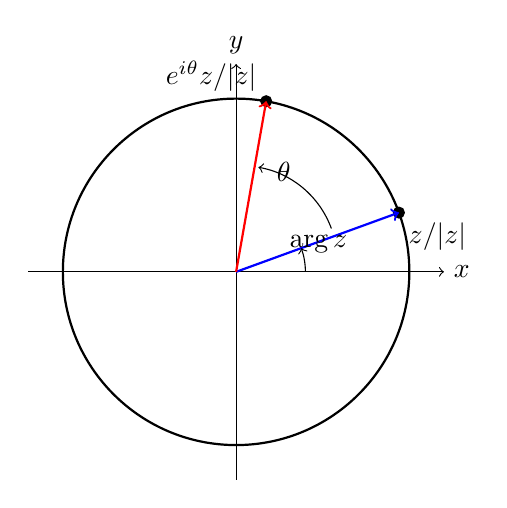
\begin{tikzpicture}[scale=1.1]
  \draw[thick] (0,0) circle (2cm);
  \draw[->] (-2.4,0)--(2.4,0) node[right] {$x$};
  \draw[->] (0,-2.4)--(0,2.4) node[above] {$y$};
  \coordinate (P) at ({2*cos(20)},{2*sin(20)});
  \coordinate (Q) at ({2*cos(20+60)},{2*sin(20+60)});
  \draw[fill=black] (P) circle (1.8pt) node[below right] {$z/|z|$};
  \draw[fill=black] (Q) circle (1.8pt) node[above left] {$e^{i\theta}z/|z|$};
  \draw[thick,->,blue] (0,0)--(P);
  \draw[thick,->,red] (0,0)--(Q);
  \draw[->] (0.8,0) arc (0:20:0.8);
  \node at (0.95,0.32) {$\arg z$};
  \draw[->] (1.1,0.5) arc (20:80:1.1);
  \node at (0.55,1.15) {$\theta$};
\end{tikzpicture}
\end{center}

\bigskip
\hrule
\bigskip

\section*{Challenge (optional)}
\begin{itemize}
  \item Prove \(e^{i\theta}\overline{z}=\overline{e^{-i\theta}z}\). Geometric meaning?
  \item Find all \(\theta\) for which rotation by \(\theta\) keeps the square with vertices \((\pm1,\pm1)\) unchanged \emph{as a set}.
\end{itemize}

\bigskip
\hrule
\bigskip

\section*{Summary and next step}
You can now (1) switch forms, (2) rotate about the origin by complex multiplication or by a matrix, and (3) rotate about any center. Next (Lesson A2) we build tiny Taylor/binomial toolkits for \(\sin,\cos,e^x\) to prepare for Fourier and \(q\)-series.

\bigskip
\hrule
\bigskip

\section*{Selected Answers}\label{answersA1}
\textbf{Practice A1}
\begin{itemize}
  \item \(z=1+i\sqrt{3}\Rightarrow r=\sqrt{1+3}=2,\ \theta=\arctan(\sqrt{3}/1)=\pi/3,\ z=2e^{i\pi/3}.\)
  \item \(z=5e^{-i\pi/3}\Rightarrow x=5\cos(-\pi/3)=\tfrac{5}{2},\ y=5\sin(-\pi/3)=-\tfrac{5\sqrt3}{2}.\)
  \item \(z=-3i\Rightarrow r=3,\ \theta=-\pi/2\) (or \(3\pi/2\) if you prefer \([0,2\pi)\)); as rectangular: \(0-3i\).
\end{itemize}

\textbf{Practice A2 \& A2M}
\begin{itemize}
  \item Rotate \(z=3\) by \(60^\circ\): \(x=3,y=0\Rightarrow x'=3\cdot\tfrac12-0= \tfrac{3}{2},\ y'=3\cdot\tfrac{\sqrt3}{2}=\tfrac{3\sqrt3}{2}\Rightarrow \tfrac{3}{2}+\tfrac{3\sqrt3}{2}i.\)
  \item Rotate \(z=-2+2i\) by \(45^\circ\):
  \[
  x'=-2\cdot\tfrac{\sqrt2}{2}-2\cdot\tfrac{\sqrt2}{2}=-2\sqrt2,\quad
  y'=-2\cdot\tfrac{\sqrt2}{2}+2\cdot\tfrac{\sqrt2}{2}=0,
  \]
  so \(z'=-2\sqrt2+0\,i\). Distance check: \(|z|=\sqrt{8}=2\sqrt{2}=|z'|\).
  \item Using \(R_\pi=\begin{psmallmatrix}-1&0\\[2pt]0&-1\end{psmallmatrix}\), any \((a,b)\mapsto(-a,-b)\) (a \(180^\circ\) half-turn).
\end{itemize}

\textbf{Practice A3}
\begin{itemize}
  \item Rotate \(z=0\) by \(120^\circ\) about \(a=-1+i\):
  \[
  z_{\text{new}}=a+e^{i2\pi/3}(0-a)
  =(-1+i)+e^{i2\pi/3}(1-i).
  \]
  Compute \(e^{i2\pi/3}=-\tfrac12+i\tfrac{\sqrt3}{2}\).
  \[
  (1-i)\cdot\Big(-\tfrac12+i\tfrac{\sqrt3}{2}\Big)
  = -\tfrac12 - i\Big(-\tfrac{\sqrt3}{2}\Big) + i\Big(-\tfrac12\Big) + i^2\Big(-\tfrac{\sqrt3}{2}\Big)
  = -\tfrac12 + i\Big(\tfrac{\sqrt3}{2}-\tfrac12\Big) + \tfrac{\sqrt3}{2}.
  \]
  So
  \[
  z_{\text{new}}=\Big(-1-\tfrac12+\tfrac{\sqrt3}{2}\Big)
  + i\Big(1+\tfrac{\sqrt3}{2}-\tfrac12\Big)
  =\Big(-\tfrac{3}{2}+\tfrac{\sqrt3}{2}\Big)
  + i\Big(\tfrac{1}{2}+\tfrac{\sqrt3}{2}\Big).
  \]
  (Any equivalent algebra earns full credit; numeric form also fine.)
  \item Rotate \(z=(2,0)\) by \(90^\circ\) about \(a=(1,1)\):
  \[
  w=z-a=(1,-1),\quad
  R_{\pi/2}=\begin{psmallmatrix}0&-1\\[1pt]1&0\end{psmallmatrix},\quad
  w'=(1,-1)\mapsto(1\cdot 0-(-1)\cdot 1,\ 1\cdot 1+(-1)\cdot 0)=(1,1).
  \]
  Translate back: \(z_{\text{new}}=a+w'=(2,2)\).
\end{itemize}

\end{document}
